% po4a: environment DndSidebar
% po4a: environment DndTable
\chapter{Races}
\DndDropCapLine{A}{visit to one of the great cities in the} worlds of Dungeons \& Dragons — Waterdeep, the Free City of Greyhawk, or even uncanny Sigil, the City of Doors — overwhelms the senses. Voices chatter in countless different languages. The smells of cooking in dozens of different cuisines mingle with the odors of crowded streets and poor sanitation. Buildings in myriad architectural styles display the diverse origins of their inhabitants.

And the people themselves—people of varying size, shape, and color, dressed in a dazzling spectrum of styles and hues—represent many different races, from diminu- tive halflings and stout dwarves to majestically beautiful elves, mingling among a variety of human ethnicities.

Scattered among the members of these more common races are the true exotics: a hulking dragonborn here, pushing his way through the crowd, and a sly tiefling there, lurking in the shadows with mischief in her eyes. A group of gnomes laughs as one of them activates a clever wooden toy that moves of its own accord. Half-elves and half-orcs live and work alongside humans, without fully belonging to the races of either of their parents. And there, well out of the sunlight, is a lone drow — a fugitive from the subterranean expanse of the Underdark, trying to make his way in a world that fears his kind. The Player’s Handbook has more information about these unusual races.

\section{Choosing a Race}
Humans are the most common people in the worlds of D\&D, but they live and work alongside dwarves, elves, halflings, and countless other fantastic species. Your character belongs to one of these peoples.

Not every intelligent race of the multiverse is appropriate for a player-controlled adventurer. Dwarves, elves, halflings, and humans are the most common races to produce the sort of adventurers who make up typical parties. Other races and subraces are less common as adventurers.

Your choice of race affects many different aspects of your character. It establishes fundamental qualities that exist throughout your character’s adventuring career. When making this decision, keep in mind the kind of character you want to play. For example, a halfling could be a good choice for a sneaky rogue, a dwarf makes a tough warrior, and an elf can be a master of arcane magic.

Your character race not only affects your ability scores and traits but also provides the cues for building your character’s story. Each race’s description in this chapter includes information to help you roleplay a character of that race, including personality, physical appearance, fea- tures of society, and racial alignment tendencies. These details are suggestions to help you think about your char- acter; adventurers can deviate widely from the norm for their race. It’s worthwhile to consider why your character is different, as a helpful way to think about your character’s background and personality.

\subsection{Racial Traits}
The description of each race includes racial traits that are common to members of that race. The following entries appear among the traits of most races.

\subsubsection{Ability Score Increase}
Every race increases one or more of a character’s ability scores.

\subsubsection{Age}
The age entry notes the age when a member of the race is considered an adult, as well as the race’s expected lifespan. This information can help you decide how old your character is at the start of the game. You can choose any age for your character, which could provide an ex- planation for some of your ability scores. For example, if you play a young or very old character, your age could explain a particularly low Strength or Constitution score, while advanced age could account for a high Intelligence or Wisdom.

\subsubsection{Alignment}
Most races have tendencies toward certain alignments, described in this entry. These are not binding for player characters, but considering why your dwarf is chaotic, for example, in defiance of lawful dwarf society can help you better define your character.

\subsubsection{Size}
Characters of most races are Medium, a size category including creatures that are roughly 4 to 8 feet tall. Members of a few races are Small (between 2 and 4 feet tall), which means that certain rules of the game affect them differently. The most important of these rules is that Small characters have trouble wielding heavy weapons, as explained in chapter 5.

\subsubsection{Speed}
Your speed determines how far you can move when traveling (chapter 8) and fighting (chapter 9).

\subsubsection{Languages}
By virtue of your race, your character can speak, read, and write certain languages. Chapter 4 lists the most common languages of the D\&D multiverse.

\subsubsection{Subraces}
Some races have subraces. Members of a subrace have the traits of the parent race in addition to the traits specified for their subrace. Relationships among subraces vary significantly from race to race and world to world. In the Dragonlance campaign setting, for example, mountain dwarves and hill dwarves live together as different clans of the same people, but in the Forgotten Realms, they live far apart in separate kingdoms and call themselves shield dwarves and gold dwarves, respectively.

\section{Dwarf}
\DndQuote%
  {``Yer late, elf!'' came the rough edge of a familiar}
  {voice. Bruenor Battlehammer walked up the back of his dead foe, disregarding the fact that the heavy monster lay on top of his elven friend. In spite of the added discomfort, the dwarf’s long, pointed, often-broken nose and gray-streaked though still-fiery red beard came as a welcome sight to Drizzt. ``Knew I’d find ye in trouble if I came out an’ looked for ye!''}
  {R. A. Salvatore, The Crystal Shard}

\ \newline
\par\noindent Kingdoms rich in ancient grandeur, halls carved into the roots of mountains, the echoing of picks and hammers in deep mines and blazing forges, a commitment to clan and tradition, and a burning hatred of goblins and orcs— these common threads unite all dwarves.

\subsection{Short and Stout}
Bold and hardy, dwarves are known as skilled warriors, miners, and workers of stone and metal. Though they stand well under 5 feet tall, dwarves are so broad and compact that they can weigh as much as a human standing nearly two feet taller. Their courage and endurance are also easily a match for any of the larger folk.

Dwarven skin ranges from deep brown to a paler hue tinged with red, but the most common shades are light brown or deep tan, like certain tones of earth. Their hair, worn long but in simple styles, is usually black, gray, or brown, though paler dwarves often have red hair. Male dwarves value their beards highly and groom them carefully.

\subsection{Long Memory, Long Grudges}
Dwarves can live to be more than 400 years old, so the oldest living dwarves often remember a very different world. For example, some of the oldest dwarves living in Citadel Felbarr (in the world of the Forgotten Realms) can recall the day, more than three centuries ago, when orcs conquered the fortress and drove them into an exile that lasted over 250 years. This longevity grants them a perspective on the world that shorter-lived races such as humans and halflings lack.

Dwarves are solid and enduring like the mountains they love, weathering the passage of centuries with stoic endurance and little change. They respect the traditions of their clans, tracing their ancestry back to the founding of their most ancient strongholds in the youth of the world, and don’t abandon those traditions lightly. Part of those traditions is devotion to the gods of the dwarves, who uphold the dwarven ideals of industrious labor, skill in battle, and devotion to the forge.

Individual dwarves are determined and loyal, true to their word and decisive in action, sometimes to the point of stubbornness. Many dwarves have a strong sense of justice, and they are slow to forget wrongs they have suffered. A wrong done to one dwarf is a wrong done to the dwarf’s entire clan, so what begins as one dwarf’s hunt for vengeance can become a full-blown clan feud.

\subsection{Clans and Kingdoms}
Dwarven kingdoms stretch deep beneath the mountains where the dwarves mine gems and precious metals and forge items of wonder. They love the beauty and artistry of precious metals and fine jewelry, and in some dwarves this love festers into avarice. Whatever wealth they can’t find in their mountains, they gain through trade. They dislike boats, so enterprising humans and halflings frequently handle trade in dwarven goods along water routes. Trustworthy members of other races are welcome in dwarf settlements, though some areas are off limits even to them.

The chief unit of dwarven society is the clan, and dwarves highly value social standing. Even dwarves who live far from their own kingdoms cherish their clan identities and affiliations, recognize related dwarves, and invoke their ancestors’ names in oaths and curses. To be clanless is the worst fate that can befall a dwarf.

Dwarves in other lands are typically artisans, especially weaponsmiths, armorers, and jewelers. Some become mercenaries or bodyguards, highly sought after for their courage and loyalty.

\subsection{Gods, Gold, and Clan}
Dwarves who take up the adventuring life might be motivated by a desire for treasure — for its own sake, for a specific purpose, or even out of an altruistic desire to help others. Other dwarves are driven by the command or inspiration of a deity, a direct calling or simply a desire to bring glory to one of the dwarf gods. Clan and ancestry are also important motivators. A dwarf might seek to restore a clan’s lost honor, avenge an ancient wrong the clan suffered, or earn a new place within the clan after having been exiled. Or a dwarf might search for the axe wielded by a mighty ancestor, lost on the field of battle centuries ago.

\begin{DndSidebar}[float=!b]{Slow to Trust}
Dwarves get along passably well with most other races. ``The difference between an acquaintance and a friend is about a hundred years,'' is a dwarf saying that might be hyperbole, but certainly points to how difficult it can be for a member of a short-lived race like humans to earn a dwarf’s trust.

\textbf{Elves.} ``It’s not wise to depend on the elves. No telling what an elf will do next; when the hammer meets the orc’s head, they’re as apt to start singing as to pull out a sword. They’re flighty and frivolous. Two things to be said for them, though: They don’t have many smiths, but the ones they have do very fine work. And when orcs or goblins come streaming down out of the mountains, an elf’s good to have at your back. Not as good as a dwarf, maybe, but no doubt they hate the orcs as much as we do.''

\textbf{Halflings.} ``Sure, they’re pleasant folk. But show me a halfling hero. An empire, a triumphant army. Even a treasure for the ages made by halfling hands. Nothing. How can you take them seriously?''

\textbf{Humans.} ``You take the time to get to know a human, and by then the human’s on her deathbed. If you’re lucky, she’s got kin—a daughter or granddaughter, maybe—who’s got hands and heart as good as hers. That’s when you can make a human friend. And watch them go! They set their hearts on something, they’ll get it, whether it’s a dragon’s hoard or an empire’s throne. You have to admire that kind of dedication, even if it gets them in trouble more often than not.''
\end{DndSidebar}

\subsection{Dwarf Names}
A dwarf’s name is granted by a clan elder, in accordance with tradition. Every proper dwarven name has been used and reused down through the generations. A dwarf’s name belongs to the clan, not to the individual. A dwarf who misuses or brings shame to a clan name is stripped of the name and forbidden by law to use any dwarven name in its place.

\ \newline
\noindent \textbf{Male Names:} \hangindent=0.3cm Adrik, Alberich, Baern, Barendd, Brottor, Bruenor, Dain, Darrak, Delg, Eberk, Einkil, Fargrim, Flint, Gardain, Harbek, Kildrak, Morgran, Orsik, Oskar, Rangrim, Rurik, Taklinn, Thoradin, Thorin, Tordek, Traubon, Travok, Ulfgar, Veit, Vondal

\noindent \textbf{Female Names:} \hangindent=0.3cm Amber, Artin, Audhild, Bardryn, Dagnal, Diesa, Eldeth, Falkrunn, Finellen, Gunnloda, Gurdis, Helja, Hlin, Kathra, Kristryd, Ilde, Liftrasa, Mardred, Riswynn, Sannl, Torbera, Torgga, Vistra

\noindent \textbf{Clan Names:} \hangindent=0.3cm Balderk, Battlehammer, Brawnanvil, Dankil, Fireforge, Frostbeard, Gorunn, Holderhek, Ironfist, Loderr, Lutgehr, Rumnaheim, Strakeln, Torunn, Ungart

\subsection{Dwarf Traits}
Your dwarf character has an assortment of inborn abilities, part and parcel of dwarven nature.

\textbf{Ability Score Increase.} Your Constitution score in- creases by 2.

\textbf{Age.} Dwarves mature at the same rate as humans, but they’re considered young until they reach the age of 50. On average, they live about 350 years.

\textbf{Alignment.} Most dwarves are lawful, believing firmly in the benefits of a well-ordered society. They tend toward good as well, with a strong sense of fair play and a belief that everyone deserves to share in the benefits of a just order.

\textbf{Size.} Dwarves stand between 4 and 5 feet tall and aver- age about 150 pounds. Your size is Medium.

\textbf{Speed.} Your base walking speed is 25 feet. Your speed is not reduced by wearing heavy armor.

\textbf{Darkvision.} Accustomed to life underground, you have superior vision in dark and dim conditions. You can see in dim light within 60 feet of you as if it were bright light, and in darkness as if it were dim light. You can’t discern color in darkness, only shades of gray.

\textbf{Dwarven Resilience.} You have advantage on saving throws against poison, and you have resistance against poison damage (explained in chapter 9).

\textbf{Dwarven Combat Training.} You have proficiency with the battleaxe, handaxe, light hammer, and warhammer.

\textbf{Tool Proficiency.} You gain proficiency with the artisan’s tools of your choice: smith’s tools, brewer’s supplies, or mason’s tools.

\textbf{Stonecunning.} Whenever you make an Intelligence (History) check related to the origin of stonework, you are considered proficient in the History skill and add double your proficiency bonus to the check, instead of your nor- mal proficiency bonus.

\textbf{Languages.} You can speak, read, and write Common and Dwarvish. Dwarvish is full of hard consonants and guttural sounds, and those characteristics spill over into whatever other language a dwarf might speak.

\textbf{Subrace.} Two main subraces of dwarves populate the worlds of D\&D: hill dwarves and mountain dwarves. Choose one of these subraces.

\begin{DndSidebar}[float=!t]{Duergar}
In cities deep in the Underdark live the duergar, or gray dwarves. These vicious, stealthy slave traders raid the surface world for captives, then sell their prey to the other races of the Underdark. They have innate magical abilities to become invisible and to temporarily grow to giant size.
\end{DndSidebar}

\subsubsection{Hill Dwarf}
As a hill dwarf, you have keen senses, deep intuition, and remarkable resilience. The gold dwarves of Faerûn in their mighty southern kingdom are hill dwarves, as are the exiled Neidar and the debased Klar of Krynn in the Dragonlance setting.

\textbf{Ability Score Increase.} Your Wisdom score increases by 1.

\textbf{Dwarven Toughness.} Your hit point maximum increases by 1, and it increases by 1 every time you gain a level.

\subsubsection{Mountain Dwarf}
As a mountain dwarf, you’re strong and hardy, accus- tomed to a difficult life in rugged terrain. You’re probably on the tall side (for a dwarf), and tend toward lighter coloration. The shield dwarves of northern Faerûn, as well as the ruling Hylar clan and the noble Daewar clan of Dragonlance, are mountain dwarves.

\textbf{Ability Score Increase.} Your Strength score increases by 2.

\textbf{Dwarven Armor Training.} You have proficiency with light and medium armor.

\vspace*{\fill}

\section{Elf}
\DndQuote%
  {``I have never imagined such beauty existed,''}
  {Goldmoon said softly. The day’s march had been difficult, but the reward at the end was beyond their dreams. The companions stood on a high cliff over the fabled city of Qualinost. \newline\indent Four slender spires rose from the city’s corners like glistening spindles, their brilliant white stone marbled with shining silver. Graceful arches, swooping from spire to spire, soared through the air. Crafted by ancient dwarven metalsmiths, they were strong enough to hold the weight of an army, yet they appeared so delicate that a bird lighting on them might overthrow the balance. These glistening arches were the city’s only boundaries; there was no wall around Qualinost. The elven city opened its arms lovingly to the wilderness.}
  {Margaret Weis \& Tracy Hickman,\newline\hspace*{\fill} Dragons of Autumn Twilight}

\ \newline
\par\noindent Elves are a magical people of otherworldly grace, living in the world but not entirely part of it. They live in places of ethereal beauty, in the midst of ancient forests or in silvery spires glittering with faerie light, where soft music drifts through the air and gentle fragrances waft on the breeze. Elves love nature and magic, art and artistry, music and poetry, and the good things of the world.

\subsection{Slender and Graceful}
With their unearthly grace and fine features, elves appear hauntingly beautiful to humans and members of many other races. They are slightly shorter than humans on average, ranging from well under 5 feet tall to just over 6 feet. They are more slender than humans, weighing only 100 to 145 pounds. Males and females are about the same height, and males are only marginally heavier than females.

Elves’ coloration encompasses the normal human range and also includes skin in shades of copper, bronze, and almost bluish-white, hair of green or blue, and eyes like pools of liquid gold or silver. Elves have no facial and little body hair. They favor elegant clothing in bright colors, and they enjoy simple yet lovely jewelry.

\subsection{A Timeless Perspective}
Elves can live well over 700 years, giving them a broad perspective on events that might trouble the shorter-lived races more deeply. They are more often amused than excited, and more likely to be curious than greedy. They tend to remain aloof and unfazed by petty happenstance. When pursuing a goal, however, whether adventuring on a mission or learning a new skill or art, elves can be focused and relentless. They are slow to make friends and enemies, and even slower to forget them. They reply to petty insults with disdain and to serious insults with vengeance.

Like the branches of a young tree, elves are flexible in the face of danger. They trust in diplomacy and com- promise to resolve differences before they escalate to violence. They have been known to retreat from intru- sions into their woodland homes, confident that they can simply wait the invaders out. But when the need arises, elves reveal a stern martial side, demonstrating skill with sword, bow, and strategy.

\subsection{Hidden Woodland Realms}
Most elves dwell in small forest villages hidden among the trees. Elves hunt game, gather food, and grow vege- tables, and their skill and magic allow them to support themselves without the need for clearing and plowing land. They are talented artisans, crafting finely worked clothes and art objects. Their contact with outsiders is usually limited, though a few elves make a good living by trading crafted items for metals (which they have no interest in mining).

Elves encountered outside their own lands are com- monly traveling minstrels, artists, or sages. Human nobles compete for the services of elf instructors to teach swordplay or magic to their children.

\begin{DndSidebar}[float=!b]{Haughty but Gracious}
Although they can be haughty, elves are generally gracious even to those who fall short of their high expectations— which is most non-elves. Still, they can find good in just about anyone.

\textbf{Dwarves.} ``Dwarves are dull, clumsy oafs. But what they lack in humor, sophistication, and manners, they make up in valor. And I must admit, their best smiths produce art that approaches elven quality.''

\textbf{Halflings.} ``Halflings are people of simple pleasures, and that is not a quality to scorn. They’re good folk, they care for each other and tend their gardens, and they have proven themselves tougher than they seem when the need arises.''

\textbf{Humans.} ``All that haste, their ambition and drive to accomplish something before their brief lives pass away— human endeavors seem so futile sometimes. But then you look at what they have accomplished, and you have to appreciate their achievements. If only they could slow down and learn some refinement.''
\end{DndSidebar}

\subsection{Exploration and Adventure}
Elves take up adventuring out of wanderlust. Since they are so long-lived, they can enjoy centuries of exploration and discovery. They dislike the pace of human society, which is regimented from day to day but constantly changing over decades, so they find careers that let them travel freely and set their own pace. Elves also enjoy exercising their martial prowess or gaining greater magical power, and adventuring allows them to do so. Some might join with rebels fighting against oppression, and others might become champions of moral causes.

\subsection{Elf Names}
Elves are considered children until they declare them- selves adults, some time after the hundredth birthday, and before this period they are called by child names.

On declaring adulthood, an elf selects an adult name, although those who knew him or her as a youngster might continue to use the child name. Each elf’s adult name is a unique creation, though it might reflect the names of respected individuals or other family members. Little distinction exists between male names and female names; the groupings here reflect only general tendencies. In addition, every elf bears a family name, typically a combination of other Elvish words. Some elves traveling among humans translate their family names into Common, but others retain the Elvish version.

\ \newline
\noindent \textbf{Child Names:} \hangindent=0.3cm Ara, Bryn, Del, Eryn, Faen, Innil, Lael, Mella, Naill, Naeris, Phann, Rael, Rinn, Sai, Syllin, Thia, Vall

\noindent \textbf{Male Adult Names:} \hangindent=0.3cm Adran, Aelar, Aramil, Arannis, Aust, Beiro, Berrian, Carric, Enialis, Erdan, Erevan, Galinndan, Hadarai, Heian, Himo, Immeral, Ivellios, Laucian, Mindartis, Paelias, Peren, Quarion, Riardon, Rolen, Soveliss, Thamior, Tharivol, Theren, Varis

\noindent \textbf{Female Adult Names:} \hangindent=0.3cm Adrie, Althaea, Anastrianna, Andraste, Antinua, Bethrynna, Birel, Caelynn, Drusilia, Enna, Felosial, Ielenia, Jelenneth, Keyleth, Leshanna, Lia, Meriele, Mialee, Naivara, Quelenna, Quillathe, Sariel, Shanairra, Shava, Silaqui, Theirastra, Thia, Vadania, Valanthe, Xanaphia

\noindent \textbf{Family Names (Common Translations)} \hangindent=0.3cm Amakiir (Gemflower), Amastacia (Starflower), Galanodel (Moonwhisper), Holimion (Diamonddew), Ilphelkiir (Gemblossom), Liadon (Silverfrond), Meliamne (Oakenheel), Naïlo (Nightbreeze), Siannodel (Moonbrook), Xiloscient (Goldpetal)

\subsection{Elf Traits}
Your elf character has a variety of natural abilities, the result of thousands of years of elven refinement.

\textbf{Ability Score Increase.} Your Dexterity score in- creases by 2.

\textbf{Age.} Although elves reach physical maturity at about the same age as humans, the elven understanding of adulthood goes beyond physical growth to encompass worldly experience. An elf typically claims adulthood and an adult name around the age of 100 and can live to be 750 years old.

\textbf{Alignment.} Elves love freedom, variety, and self-ex- pression, so they lean strongly toward the gentler aspects of chaos. They value and protect others’ freedom as well as their own, and they are more often good than not.

\textbf{Size.} Elves range from under 5 to over 6 feet tall and have slender builds. Your size is Medium.

\textbf{Speed.} Your base walking speed is 30 feet.

\textbf{Darkvision.} Accustomed to twilit forests and the night sky, you have superior vision in dark and dim conditions. You can see in dim light within 60 feet of you as if it were bright light, and in darkness as if it were dim light. You can’t discern color in darkness, only shades of gray.

\textbf{Keen Senses.} You have proficiency in the Percep- tion skill.

\textbf{Fey Ancestry.} You have advantage on saving throws against being charmed, and magic can’t put you to sleep.

\textbf{Trance.} Elves don’t need to sleep. Instead, they meditate deeply, remaining semiconscious, for 4 hours a day. (The Common word for such meditation is ``trance.'') While meditating, you can dream after a fashion; such dreams are actually mental exercises that have become reflexive through years of practice. After resting in this way, you gain the same benefit that a human does from 8 hours of sleep.

\textbf{Languages.} You can speak, read, and write Common and Elvish. Elvish is fluid, with subtle intonations and intricate grammar. Elven literature is rich and varied, and their songs and poems are famous among other races. Many bards learn their language so they can add Elvish ballads to their repertoires.

\begin{DndSidebar}[float=!b]{The Darkness of the Drow}
Were it not for one renowned exception, the race of drow would be universally reviled. Their depraved society is preoccupied with the favor of Lolth, their spider-goddess, who sanctions murder and the extermination of entire families as noble houses vie for position. Drow grow
up believing that surface-dwelling races are worthless except as slaves.

Yet one drow, at least, broke the mold. In the world of the Forgotten Realms, Drizzt Do’Urden, ranger of the North, has proven his quality as a good-hearted defender of the weak and innocent.
\end{DndSidebar}

\textbf{Subrace.} Ancient divides among the elven people resulted in three main subraces: high elves, wood elves, and dark elves, who are commonly called drow. This document presents two of these subraces to choose from. In some worlds, these subraces are divided still further (such as the sun elves and moon elves of the Forgotten Realms), so if you wish, you can choose a narrower subrace.

\subsubsection{High Elf}
As a high elf, you have a keen mind and a mastery of at least the basics of magic. In many of the worlds of D\&D, there are two kinds of high elves. One type (which includes the gray elves and valley elves of Greyhawk, the Silvanesti of Dragonlance, and the sun elves of the Forgotten Realms) is haughty and reclusive, believing themselves to be superior to non-elves and even other elves. The other type (including the high elves of Greyhawk, the Qualinesti of Dragonlance, and the moon elves of the Forgotten Realms) are more common and more friendly, and often encountered among humans and other races.

The sun elves of Faerûn (also called gold elves or sun- rise elves) have bronze skin and hair of copper, black, or golden blond. Their eyes are golden, silver, or black. Moon elves (also called silver elves or gray elves) are much paler, with alabaster skin sometimes tinged with blue. They often have hair of silver-white, black, or blue, but various shades of blond, brown, and red are not uncommon. Their eyes are blue or green and flecked with gold.

\textbf{Ability Score Increase.} Your Intelligence score in- creases by 1.

\textbf{Elf Weapon Training.} You have proficiency with the longsword, shortsword, shortbow, and longbow.

\textbf{Cantrip.} You know one cantrip of your choice from the wizard spell list. Intelligence is your spellcasting ability for it.

\textbf{Extra Language.} You can speak, read, and write one extra language of your choice.

\subsubsection{Wood Elf}
As a wood elf, you have keen senses and intuition, and your fleet feet carry you quickly and stealthily through your native forests. This category includes the wild elves (grugach) of Greyhawk and the Kagonesti of Dragonlance, as well as the races called wood elves in Greyhawk and the Forgotten Realms. In Faerûn, wood elves (also called wild elves, green elves, or forest elves) are reclusive and distrusting of non-elves.

Wood elves’ skin tends to be copperish in hue, sometimes with traces of green. Their hair tends toward browns and blacks, but it is occasionally blond or copper-colored. Their eyes are green, brown, or hazel.

\textbf{Ability Score Increase.} Your Wisdom score increases by 1.

\textbf{Elf Weapon Training.} You have proficiency with the longsword, shortsword, shortbow, and longbow.

\textbf{Fleet of Foot.} Your base walking speed increases to 35 feet.

\textbf{Mask of the Wild.} You can attempt to hide even when you are only lightly obscured by foliage, heavy rain, falling snow, mist, and other natural phenomena.

\section{Halfling}

\DndQuote%
  {Regis the halfling, the only one of his kind for}
  {hundreds of miles in any direction, locked his fingers behind his head and leaned back against the mossy blanket of the tree trunk. Regis was short, even by the standards of his diminutive race, with the fluff of his curly brown locks barely cresting the three-foot mark, but his belly was amply thick- ened by his love of a good meal, or several, as the opportu- nities presented themselves. The crooked stick that served as his fishing pole rose up above him, clenched between two of his toes, and hung out over the quiet lake, mirrored perfectly in the glassy surface of Maer Dualdon.}
  {R.A. Salvatore, The Crystal Shard}

\ \newline
\par\noindent The comforts of home are the goals of most halflings’ lives: a place to settle in peace and quiet, far from ma- rauding monsters and clashing armies; a blazing fire and a generous meal; fine drink and fine conversation. Though some halflings live out their days in remote agricultural communities, others form nomadic bands that travel constantly, lured by the open road and the wide horizon to discover the wonders of new lands and peoples. But even these wanderers love peace, food, hearth, and home, though home might be a wagon jostling along an dirt road or a raft floating downriver.

\subsection{Small and Practical}
The diminutive halflings survive in a world full of larger creatures by avoiding notice or, barring that, avoiding offense. Standing about 3 feet tall, they appear relatively harmless and so have managed to survive for centuries in the shadow of empires and on the edges of wars and political strife. They are inclined to be stout, weighing between 40 and 45 pounds.

Halflings’ skin ranges from tan to pale with a ruddy cast, and their hair is usually brown or sandy brown and wavy. They have brown or hazel eyes. Halfling men often sport long sideburns, but beards are rare among them and mustaches even more so. They like to wear simple, comfortable, and practical clothes, favoring bright colors.

Halfling practicality extends beyond their clothing. They’re concerned with basic needs and simple pleasures and have little use for ostentation. Even the wealthiest of halflings keep their treasures locked in a cellar rather than on display for all to see. They have a knack for finding the most straightforward solution to a problem, and have little patience for dithering.

\subsection{Kind and Curious}
Halflings are an affable and cheerful people. They cherish the bonds of family and friendship as well as the comforts of hearth and home, harboring few dreams of gold or glory. Even adventurers among them usually venture into the world for reasons of community, friendship, wanderlust, or curiosity. They love discovering new things, even simple things, such as an exotic food or an unfamiliar style of clothing.

Halflings are easily moved to pity and hate to see any living thing suffer. They are generous, happily sharing what they have even in lean times.

\subsection{Blend into the Crowd}
Halflings are adept at fitting into a community of humans, dwarves, or elves, making themselves valuable and welcome. The combination of their inherent stealth and their unassuming nature helps halflings to avoid un- wanted attention.

Halflings work readily with others, and they are loyal to their friends, whether halfling or otherwise. They can display remarkable ferocity when their friends, families, or communities are threatened.

\subsection{Pastoral Pleasantries}
Most halflings live in small, peaceful communities with large farms and well-kept groves. They rarely build kingdoms of their own or even hold much land beyond their quiet shires. They typically don’t recognize any sort of halfling nobility or royalty, instead looking to family elders to guide them. Families preserve their traditional ways despite the rise and fall of empires.

Many halflings live among other races, where the halflings’ hard work and loyal outlook offer them abundant rewards and creature comforts. Some halfling communities travel as a way of life, driving wagons or guiding boats from place to place and maintaining no permanent home.

\subsection{Exploring Opportunities}
Halflings usually set out on the adventurer’s path to defend their communities, support their friends, or explore a wide and wonder-filled world. For them, adventuring is less a career than an opportunity or sometimes a necessity.

\subsection{Halfling Names}
A halfling has a given name, a family name, and possibly a nickname. Family names are often nicknames that stuck so tenaciously they have been passed down through the generations.

\ \newline
\noindent \textbf{Male Names:} \hangindent=0.3cm Alton, Ander, Cade, Corrin, Eldon, Errich, Finnan, Garret, Lindal, Lyle, Merric, Milo, Osborn, Perrin, Reed, Roscoe, Wellby

\noindent \textbf{Female Names:} \hangindent=0.3cm Andry, Bree, Callie, Cora, Euphemia, Jillian, Kithri, Lavinia, Lidda, Merla, Nedda, Paela, Portia, Seraphina, Shaena, Trym, Vani, Verna

\noindent \textbf{Family Names:} \hangindent=0.3cm Brushgather, Goodbarrel, Greenbottle, High-hill, Hilltopple, Leagallow, Tealeaf, Thorngage, Tosscobble, Underbough

\subsection{Halfling Traits}
Your halfling character has a number of traits in common with all other halflings.

\textbf{Ability Score Increase.} Your Dexterity score in- creases by 2.

\textbf{Age.} A halfling reaches adulthood at the age of 20 and generally lives into the middle of his or her second century.

\textbf{Alignment.} Most halflings are lawful good. As a rule, they are good-hearted and kind, hate to see others in pain, and have no tolerance for oppression. They are also very orderly and traditional, leaning heavily on the support of their community and the comfort of their old ways.

\textbf{Size.} Halflings average about 3 feet tall and weigh about 40 pounds. Your size is Small.

\textbf{Speed.} Your base walking speed is 25 feet.

\textbf{Lucky.} When you roll a 1 on the d20 for an attack roll, ability check, or saving throw, you can reroll the die and must use the new roll.

\textbf{Brave.} You have advantage on saving throws against being frightened.

\textbf{Halfling Nimbleness.} You can move through the space of any creature that is of a size larger than yours.

\textbf{Languages.} You can speak, read, and write Common and Halfling. The Halfling language isn’t secret, but halflings are loath to share it with others. They write very little, so they don’t have a rich body of literature. Their oral tradition, however, is very strong. Almost all halflings speak Common to converse with the people in whose lands they dwell or through which they are traveling.

\textbf{Subrace.} The two main kinds of halfling, lightfoot and stout, are more like closely related families than true sub- races. Choose one of these subraces.

\subsubsection{Lightfoot}
As a lightfoot halfling, you can easily hide from notice, even using other people as cover. You’re inclined to be affable and get along well with others. In the Forgotten Realms, lightfoot halflings have spread the farthest and thus are the most common variety.

Lightfoots are more prone to wanderlust than other hal- flings, and often dwell alongside other races or take up a nomadic life. In the world of Greyhawk, these halflings are called hairfeet or tallfellows.

\textbf{Ability Score Increase.} Your Charisma score in- creases by 1.

\textbf{Naturally Stealthy.} You can attempt to hide even when you are obscured only by a creature that is at least one size larger than you.

\subsubsection{Stout}
As a stout halfling, you’re hardier than average and have some resistance to poison. Some say that stouts have dwarven blood. In the Forgotten Realms, these halflings are called stronghearts, and they’re most common in the south.

\textbf{Ability Score Increase.} Your Constitution score in- creases by 1.

\textbf{Stout Resilience.} You have advantage on saving throws against poison, and you have resistance against poison damage.

\begin{DndSidebar}[float=!t]{Affable and Positive}
Halflings try to get along with everyone else and are loath to make sweeping generalizations—especially negative ones.

\textbf{Dwarves.} ``Dwarves make loyal friends, and you can count on them to keep their word. But would it hurt them to smile once in a while?''

\textbf{Elves.} ``They’re so beautiful! Their faces, their music, their grace and all. It’s like they stepped out of a wonderful dream. But there’s no telling what’s going on behind their smiling faces — surely more than they ever let on.''

\textbf{Humans.} ``Humans are a lot like us, really. At least some of them are. Step out of the castles and keeps, go talk to the farmers and herders and you’ll find good, solid folk. Not that there’s anything wrong with the barons and soldiers— you have to admire their conviction. And by protecting their own lands, they protect us as well.''
\end{DndSidebar}

\section{Human}
\DndQuote%
  {These were the stories of a restless people who}
  {long ago took to the seas and rivers in longboats, first to pillage and terrorize, then to settle. Yet there was an energy, a love of adventure, that sang from every page. Long into the night Liriel read, lighting candle after precious candle. \newline\indent She’d never given much thought to humans, but these sto- ries fascinated her. In these yellowed pages were tales of bold heroes, strange and fierce animals, mighty primitive gods, and a magic that was part and fabric of that distant land.}
  {Elaine Cunningham, Daughter of the Drow}

\ \newline
\par\noindent In the reckonings of most worlds, humans are the young- est of the common races, late to arrive on the world scene and short-lived in comparison to dwarves, elves, and dragons. Perhaps it is because of their shorter lives that they strive to achieve as much as they can in the years they are given. Or maybe they feel they have something to prove to the elder races, and that’s why they build their mighty empires on the foundation of conquest and trade. Whatever drives them, humans are the innovators, the achievers, and the pioneers of the worlds.

\subsection{A Broad Spectrum}
With their penchant for migration and conquest, humans are more physically diverse than other common races. There is no typical human. An individual can stand from 5 feet to a little over 6 feet tall and weigh from 125 to 250 pounds. Human skin shades range from nearly black to very pale, and hair colors from black to blond (curly, kinky, or straight); males might sport facial hair that is sparse or thick. A lot of humans have a dash of nonhuman blood, revealing hints of elf, orc, or other lineages. Humans reach adulthood in their late teens and rarely live even a single century.

\subsection{Variety in All Things}
Humans are the most adaptable and ambitious people among the common races. They have widely varying tastes, morals, and customs in the many different lands where they have settled. When they settle, though, they stay: they build cities to last for the ages, and great kingdoms that can persist for long centuries. An individual human might have a relatively short life span, but a hu- man nation or culture preserves traditions with origins far beyond the reach of any single human’s memory. They live fully in the present—making them well suited to the adventuring life — but also plan for the future, striving to leave a lasting legacy. Individually and as a group, humans are adaptable opportunists, and they stay alert to changing political and social dynamics.

\subsection{Lasting Institutions}
Where a single elf or dwarf might take on the responsibility of guarding a special location or a powerful secret, humans found sacred orders and institutions for such purposes. While dwarf clans and halfling elders pass on the ancient traditions to each new generation, human temples, governments, libraries, and codes of law fix their traditions in the bedrock of history. Humans dream of immortality, but (except for those few who seek undeath or divine ascension to escape death’s clutches) they achieve it by ensuring that they will be remembered when they are gone.

Although some humans can be xenophobic, in general their societies are inclusive. Human lands welcome large numbers of nonhumans compared to the proportion of humans who live in nonhuman lands.

\subsection{Exemplars of Ambition}
Humans who seek adventure are the most daring and ambitious members of a daring and ambitious race. They seek to earn glory in the eyes of their fellows by amassing power, wealth, and fame. More than other people, humans champion causes rather than territories or groups.

\subsection{Human Names and Ethnicities}
Having so much more variety than other cultures, humans as a whole have no typical names. Some human parents give their children names from other languages, such as Dwarvish or Elvish (pronounced more or less correctly), but most parents give names that are linked to their region’s culture or to the naming traditions of their ancestors.

The material culture and physical characteristics of humans can change wildly from region to region. In the Forgotten Realms, for example, the clothing, architecture, cuisine, music, and literature are different in the northwestern lands of the Silver Marches than in distant Turmish or Impiltur to the east — and even more distinctive in far-off Kara-Tur. Human physical characteristics, though, vary according to the ancient migrations of the earliest humans, so that the humans of the Silver Marches have every possible variation of coloration
and features.

\begin{DndSidebar}[float=!b]{Everyone’s Second-Best Friends}
Just as readily as they mix with each other, humans mingle with members of other races. They get along with almost everyone, though they might not be close to many. Humans serve as ambassadors, diplomats, magistrates, merchants, and functionaries of all kinds.

\textbf{Dwarves.} ``They’re stout folk, stalwart friends, and true to their word. Their greed for gold is their downfall, though.''

\textbf{Elves.} ``It’s best not to wander into elven woods. They don’t like intruders, and you’ll as likely be bewitched as peppered with arrows. Still, if an elf can get past that damned racial pride and actually treat you like an equal, you can learn a lot from them.''

\textbf{Halflings.} ``It’s hard to beat a meal in a halfling home, as long as you don’t crack your head on the ceiling—good food and good stories in front of a nice, warm fire. If halflings had a shred of ambition, they might really amount to something.''
\end{DndSidebar}

In the Forgotten Realms, nine human ethnic groups are widely recognized, though over a dozen others are found in more localized areas of Faerûn. These groups, and the typical names of their members, can be used as inspiration no matter which world your human is in.

\subsubsection{Calishite}
Shorter and slighter in build than most other humans, Calishites have dusky brown skin, hair, and eyes. They’re found primarily in southwest Faerûn.

\ \newline
\noindent \textbf{Calishite Names:} \hangindent=0.3cm (Male) Aseir, Bardeid, Haseid, Khemed, Mehmen, Sudeiman, Zasheir; (female) Atala, Ceidil, Hama, Jasmal, Meilil, Seipora, Yasheira, Zasheida; (surnames) Basha, Dumein, Jassan, Khalid, Mostana, Pashar, Rein

\subsubsection{Chondathan}
Chondathans are slender, tawny-skinned folk with brown hair that ranges from almost blond to almost black. Most are tall and have green or brown eyes, but these traits are hardly universal. Humans of Chondathan descent dominate the central lands of Faerûn, around the Inner Sea.

\ \newline
\noindent \textbf{Chondathan Names:} \hangindent=0.3cm (Male) Darvin, Dorn, Evendur, Gorstag, Grim, Helm, Malark, Morn, Randal, Stedd; (female) Arveene, Esvele, Jhessail, Kerri, Lureene, Miri, Rowan, Shandri, Tessele; (surnames) Amblecrown, Buckman, Dundragon, Evenwood, Greycastle, Tallstag

\subsubsection{Damaran}
Found primarily in the northwest of Faerûn, Damarans are of moderate height and build, with skin hues ranging from tawny to fair. Their hair is usually brown or black, and their eye color varies widely, though brown is most common.

\ \newline
\noindent \textbf{Damaran Names:} \hangindent=0.3cm (Male) Bor, Fodel, Glar, Grigor, Igan, Ivor, Kosef, Mival, Orel, Pavel, Sergor; (female) Alethra, Kara, Katernin, Mara, Natali, Olma, Tana, Zora; (surnames) Bersk, Chernin, Dotsk, Kulenov, Marsk, Nemetsk, Shemov, Starag

\subsubsection{Illuskan}
Illuskans are tall, fair-skinned folk with blue or steely gray eyes. Most have raven-black hair, but those who inhabit the extreme northwest have blond, red, or light brown hair.

\ \newline
\noindent \textbf{Illuskan Names:} \hangindent=0.3cm (Male) Ander, Blath, Bran, Frath, Geth, Lander, Luth, Malcer, Stor, Taman, Urth; (female) Amafrey, Betha, Cefrey, Kethra, Mara, Olga, Silifrey, Westra; (surnames) Brightwood, Helder, Hornraven, Lackman, Stormwind, Windrivver

\subsubsection{Mulan}
Dominant in the eastern and southeastern shores of the Inner Sea, the Mulan are generally tall, slim, and amber- skinned, with eyes of hazel or brown. Their hair ranges from black to dark brown, but in the lands where the Mulan are most prominent, nobles and many other Mulan shave off all their hair.

\ \newline
\noindent \textbf{Mulan Names:} \hangindent=0.3cm (Male) Aoth, Bareris, Ehput-Ki, Kethoth, Mumed, Ramas, So-Kehur, Thazar-De, Urhur; (female) Arizima, Chathi, Nephis, Nulara, Murithi, Sefris, Thola, Umara, Zolis; (surnames) Ankhalab, Anskuld, Fezim, Hahpet, Nathandem, Sepret, Uuthrakt

\subsubsection{Rashemi}
Most often found east of the Inner Sea and often intermingled with the Mulan, Rashemis tend to be short, stout, and muscular. They usually have dusky skin, dark eyes, and thick black hair.

\ \newline
\noindent \textbf{Rashemi Names:} \hangindent=0.3cm (Male) Borivik, Faurgar, Jandar, Kanithar, Madislak, Ralmevik, Shaumar, Vladislak; (female) Fyevarra, Hulmarra, Immith, Imzel, Navarra, Shevarra, Tammith, Yuldra; (surnames) Chergoba, Dyernina, Iltazyara, Murnyethara, Stayanoga, Ulmokina

\subsubsection{Shou}
The Shou are the most numerous and powerful ethnic group in Kara-Tur, far to the east of Faerûn. They are yellowish-bronze in hue, with black hair and dark eyes. Shou surnames are usually presented before the given name.

\ \newline
\noindent \textbf{Shou Names:} \hangindent=0.3cm (Male) An, Chen, Chi, Fai, Jiang, Jun, Lian, Long, Meng, On, Shan, Shui, Wen; (female) Bai, Chao, Jia, Lei, Mei, Qiao, Shui, Tai; (surnames) Chien, Huang, Kao, Kung, Lao, Ling, Mei, Pin, Shin, Sum, Tan, Wan

\subsubsection{Tethyrian}
Widespread along the entire Sword Coast at the western edge of Faerûn, Tethyrians are of medium build and height, with dusky skin that tends to grow fairer the farther north they dwell. Their hair and eye color varies widely, but brown hair and blue eyes are the most common. Tethyrians primarily use Chondathan names.

\subsubsection{Turami}
Native to the southern shore of the Inner Sea, the Turami people are generally tall and muscular, with dark mahogany skin, curly black hair, and dark eyes.

\ \newline
\noindent \textbf{Turami Names:} \hangindent=0.3cm (Male) Anton, Diero, Marcon, Pieron, Rimardo, Romero, Salazar, Umbero; (female) Balama, Dona, Faila, Jalana, Luisa, Marta, Quara, Selise, Vonda; (surnames) Agosto, Astorio, Calabra, Domine, Falone, Marivaldi, Pisacar, Ramondo

\subsection{Human Traits}
It’s hard to make generalizations about humans, but your human character has these traits.

\textbf{Ability Score Increase.} Your ability scores each in- crease by 1.

\textbf{Age.} Humans reach adulthood in their late teens and live less than a century.

\textbf{Alignment.} Humans tend toward no particular alignment. The best and the worst are found among them.

\textbf{Size.} Humans vary widely in height and build, from barely 5 feet to well over 6 feet tall. Regardless of your position in that range, your size is Medium.

\textbf{Speed.} Your base walking speed is 30 feet.

\textbf{Languages.} You can speak, read, and write Common and one extra language of your choice. Humans typically learn the languages of other peoples they deal with, including obscure dialects. They are fond of sprinkling their speech with words borrowed from other tongues: Orc curses, Elvish musical expressions, Dwarvish military phrases, and so on.

\begin{DndSidebar}[float=!b]{Variant Human Traits}
If your campaign uses the optional feat rules from chapter 6 of the Player’s Handbook, your Dungeon Master might allow these variant traits, all of which replace the human’s Ability Score Increase trait.

\textbf{Ability Score Increase.} Two different ability scores of your choice increase by 1.

\textbf{Skills.} You gain proficiency in one skill of your choice.

\textbf{Feat.} You gain one feat of your choice.
\end{DndSidebar}

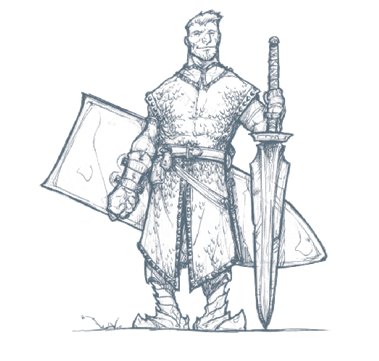
\includegraphics{img/races01.png}
